\documentclass[a4paper,10pt]{article}
\usepackage[utf8x]{inputenc}
\usepackage[T1]{fontenc}
\usepackage[bulgarian]{babel}
\usepackage{graphicx}
\usepackage{alltt}

%opening
\title{Многомерни и битови индекси. Дървовидни структури за многомерни данни в MySQL}
\author{Валентина Динкова, ф.н.71112}

\begin{document}
\maketitle

\newpage
\section{GIS и разширението на MySQL за пространствени данни}
\textbf{GIS} означава Географска Информационна Система и е един от най-очевидните примери за пространствени данни.
От там идва и главната инициатива в БД да се пазят многомерни данни.
\\
\textbf{OGC} (Open Geospatial Consorcium) е организация, която работи по стандартизирането на различни области на GIS.
Един такъв стандарт е и спецификацията за SQL, която определя разширението на SQL базирани релационни бази данни,
 което да използва GIS обекти и операции.
\\
\\
 OGC работи в 4 важни области:
\begin{itemize}
 \item типове данни;
 \item операции;
 \item възможност да се подават като вход и да се извеждат GIS данни;
 \item индексиране на пространствени данни.
\end{itemize}
Друга важна област са метаданните. Може да се пазят например данни за координатната система. MySQL за момента поддържа само 
декартовата координатната система.
\\
\section{Стандартът, използван от почти всички SQL бази данни с пространствено разширение, включително и MySQL OpenGIS}
Тук са показани типовете от стандарта.
\begin{center}
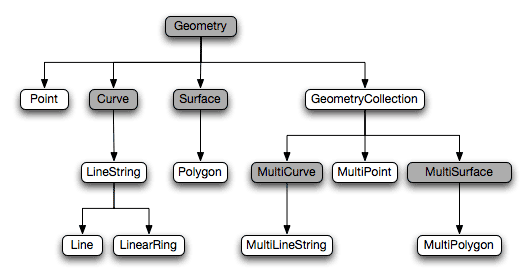
\includegraphics[width=90mm]{gis-datatypes.png}\end{center}
Типовете, отбелязани в сиво са абстракти и обекти от тези типове не могат да се създават. Това не означава, че не може да 
имаме атрибут от този тип, а че не можем да слагаме стойности от този тип в дадената колона. Например можем да 
създадем атрибут от тип Geometry и да пазим стойности от тип Point.

\section{Пространствени индекси}
Пространствените данни могат да се индексират също както останалите данни в MySQL. Но за да бъде 
индексирането ефективно, се използва пространствен тип индексиране, реализирано чрез R-дървета. 
MySQL използва R-дървета с квадратично разделяне. \\
Не всички engine-и поддържат многомерни индекси. Единствено MyISAM ги поддържа за MySQL. Той е и engine-а, с който 
по подразбиране идва MySQL.

\subsection{R-дървета}
R-дърветата (регионални дървета) са структури от данни, които наподобяват B-дърветата и се използват за многомерни данни.
Корените на R-дървото отговарят на региони, които обикновено в практиката са правоъгълници или други прости форми. 
Вместо ключове, R-дървото има подрегиони, които представят съдърванието на дъщерните си корени.
\begin{center}
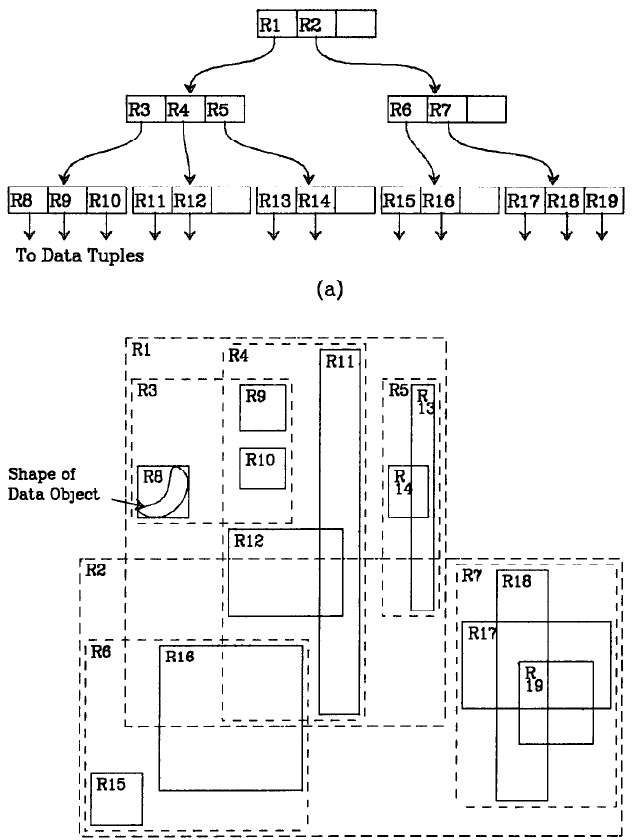
\includegraphics[width=100mm]{rtree.png}\end{center}

\subsection{R-дървета с квадратично разделяне}
При добавяне на нов запис методът на квадратичното разделяне се стреми да раздели листото на дървото на малки части, 
но не гарантира, че тези части са най-малките възможни. \\
Нека сме намерили листото, където трябва да добавим новия запис и 
нека $M = $ \textit{``брoй региони в листо''}.
\begin{enumerate}
\item Избираме 2 от $M+1$ записа да бъдат първите елементи на двете нови листа, като избираме двойката,която би заела
най-много място ако и двата елемента се постават на едно място (двойката при която покриващия регион ще е най-голям).
Намираме тази двойка като от областта покриваща двата записа изваждаме самите записи и искаме тази разлика да е най-голяма.
\begin{center}
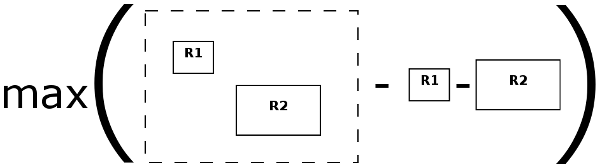
\includegraphics[width=70mm]{Diagram1.png}\end{center}
\item Останалите записи разделяме в двете листа един по един.
На всяка стъпка разширяването, необходимо за добавянето на всеки от оставащите записи към всяко листо се изчислява
и добавеният запис е този, който е показал най-голяма разлика спрямо двете листа.
\end{enumerate}

\textbf{Алгоритъмът $Quadratic Split$} разделя множество от $M+1$ индексни записа на две групи.
\begin{itemize}
 \item (Избираме първия запис за всяка група) \\
Прилагаме алгоритъма $PicSeeds$, за да изберем два записа за групите. Прибавяме всеки към съответната група.
 \item (Проверяваме дали сме приключили) \\
Ако няма повече записи за добавяне - стоп. Ако едната група има толкова малко записи, че всички останали записи трябва да 
се прибавят към нея за да има тя минималният брой, прибавяме ги и спираме.
 \item (Избираме запис, който да добавим) \\
Прилагаме алгоритъм $PickNext$,  за да изберем следващия запис който да добавим. Добавяме го към групата, чиито обграждащ 
правоъгълник се налага да бъде увиличен най-малко. Добавяме записа съм групата с по-малка област, 
след това до тази с по-малко записи, след това повтаряме от предишната стъпка.
\end{itemize}

\textbf{Алгоритъмът $PickSeeds$}
Избираме два записа да бъдат първите елементи на групите.
\begin{itemize}
 \item (Изчисляваме неефектовността за групиране) \\
За всяка двойка записи $E_{1}$ и $E_{2}$, съставяме правоъгълник $J$, който включва $E_{1}$ и $E_{2}$. 
Изчисляваме $d = area(J) - area(E_{1}) - area(E_{2})$.
\item (Избираме най-неблагоприятната двойка) \\
Избираме двойката, при която $d$ е най-голямо.
\end{itemize}

\textbf{Алгоритъмът $PickNext$}
Избираме запис, който да добавим в една от групите
\begin{itemize}
 \item (Определяме цената за прибавяне на всеки запис към всяка група) \\
За всеки запис $E$, който не е добавен, изчисляваме $d_{1} = $
областта, с която се разширява първата група при добавяне на $E$. 
По същият начин изчисляваме $d_{2}$ за втората група.
\item Избираме записа при който е максимална разликата  между $d_{1}$ и $d_{2}$.
\end{itemize}



\subsection{Примери за пространствени индекси с $MySQL$}
\textbf{Създаваме таблицата $map\_test$, където $loc$ е пространствен атрибут}. За сега все още не създаваме
пространствен индекс по него.
\begin{alltt}
mysql> create table map_test
    -> (
    ->   name varchar(100) not null primary key,
    ->   loc  geometry not null,
    -> );
Query OK, 0 rows affected (0.00 sec)
\end{alltt}

\textbf{Добавяме данни}
\begin{alltt}
mysql> insert into map_test values ('One Two', point(1,2));
Query OK, 1 row affected (0.00 sec)

mysql> insert into map_test values ('Two Two', point(2,2));
Query OK, 1 row affected (0.00 sec)

mysql> insert into map_test values ('Two One', point(2,1));
Query OK, 1 row affected (0.00 sec)
\end{alltt}

\textbf{Ето как изглежда $map\_test$ сега:}

\begin{alltt}
mysql> select name, AsText(loc) from map_test;
+---------+-------------+
| name    | AsText(loc) |
+---------+-------------+
| One Two | POINT(1 2)  |
| Two Two | POINT(2 2)  |
| Two One | POINT(2 1)  |
+---------+-------------+
3 rows in set (0.00 sec)
\end{alltt}

\textbf{Заявка за проверка коя точка се съдържа в полигона}

\begin{alltt}
mysql> SELECT name, AsText(loc) FROM map_test WHERE
    -> Contains(
    -> GeomFromText('POLYGON((0 0, 0 1, 1 1, 2 0, 0 0))'),
    -> loc) = 1;
+---------+-------------+
| name    | AsText(loc) |
+---------+-------------+
| Two One | POINT(2 1)  |
+---------+-------------+
1 row in set (0.04 sec)
\end{alltt}
Без индекс тази заявка се изпълнява за 0.04 sec

\textbf{Сега създаваме пространствен индекс по атрибута $loc$}

\begin{alltt}
mysql> create spatial index ps_index on map_test(loc);
Query OK, 3 rows affected (0.01 sec)
Records: 3  Duplicates: 0  Warnings: 0
\end{alltt}

\textbf{и отново правим същата заявка}

\begin{alltt}
mysql>  SELECT name, AsText(loc) FROM map_test WHERE
    ->  Contains(
    ->  GeomFromText('POLYGON((0 0, 0 1, 1 1, 2 0, 0 0))'),
    ->  loc) = 1;
+---------+-------------+
| name    | AsText(loc) |
+---------+-------------+
| Two One | POINT(2 1)  |
+---------+-------------+
1 row in set (0.00 sec)
\end{alltt}
Забелязва се, че когато има индекс същата заявка се изпълнява по-бързо.
\end{document}
